\documentclass[]{article}
\usepackage{lmodern}
\usepackage{amssymb,amsmath}
\usepackage{ifxetex,ifluatex}
\usepackage{fixltx2e} % provides \textsubscript
\ifnum 0\ifxetex 1\fi\ifluatex 1\fi=0 % if pdftex
  \usepackage[T1]{fontenc}
  \usepackage[utf8]{inputenc}
\else % if luatex or xelatex
  \ifxetex
    \usepackage{mathspec}
  \else
    \usepackage{fontspec}
  \fi
  \defaultfontfeatures{Ligatures=TeX,Scale=MatchLowercase}
\fi
% use upquote if available, for straight quotes in verbatim environments
\IfFileExists{upquote.sty}{\usepackage{upquote}}{}
% use microtype if available
\IfFileExists{microtype.sty}{%
\usepackage{microtype}
\UseMicrotypeSet[protrusion]{basicmath} % disable protrusion for tt fonts
}{}
\usepackage[margin=1in]{geometry}
\usepackage{hyperref}
\hypersetup{unicode=true,
            pdftitle={hw\_2},
            pdfauthor={Mrinal Vashisth},
            pdfborder={0 0 0},
            breaklinks=true}
\urlstyle{same}  % don't use monospace font for urls
\usepackage{color}
\usepackage{fancyvrb}
\newcommand{\VerbBar}{|}
\newcommand{\VERB}{\Verb[commandchars=\\\{\}]}
\DefineVerbatimEnvironment{Highlighting}{Verbatim}{commandchars=\\\{\}}
% Add ',fontsize=\small' for more characters per line
\usepackage{framed}
\definecolor{shadecolor}{RGB}{248,248,248}
\newenvironment{Shaded}{\begin{snugshade}}{\end{snugshade}}
\newcommand{\AlertTok}[1]{\textcolor[rgb]{0.94,0.16,0.16}{#1}}
\newcommand{\AnnotationTok}[1]{\textcolor[rgb]{0.56,0.35,0.01}{\textbf{\textit{#1}}}}
\newcommand{\AttributeTok}[1]{\textcolor[rgb]{0.77,0.63,0.00}{#1}}
\newcommand{\BaseNTok}[1]{\textcolor[rgb]{0.00,0.00,0.81}{#1}}
\newcommand{\BuiltInTok}[1]{#1}
\newcommand{\CharTok}[1]{\textcolor[rgb]{0.31,0.60,0.02}{#1}}
\newcommand{\CommentTok}[1]{\textcolor[rgb]{0.56,0.35,0.01}{\textit{#1}}}
\newcommand{\CommentVarTok}[1]{\textcolor[rgb]{0.56,0.35,0.01}{\textbf{\textit{#1}}}}
\newcommand{\ConstantTok}[1]{\textcolor[rgb]{0.00,0.00,0.00}{#1}}
\newcommand{\ControlFlowTok}[1]{\textcolor[rgb]{0.13,0.29,0.53}{\textbf{#1}}}
\newcommand{\DataTypeTok}[1]{\textcolor[rgb]{0.13,0.29,0.53}{#1}}
\newcommand{\DecValTok}[1]{\textcolor[rgb]{0.00,0.00,0.81}{#1}}
\newcommand{\DocumentationTok}[1]{\textcolor[rgb]{0.56,0.35,0.01}{\textbf{\textit{#1}}}}
\newcommand{\ErrorTok}[1]{\textcolor[rgb]{0.64,0.00,0.00}{\textbf{#1}}}
\newcommand{\ExtensionTok}[1]{#1}
\newcommand{\FloatTok}[1]{\textcolor[rgb]{0.00,0.00,0.81}{#1}}
\newcommand{\FunctionTok}[1]{\textcolor[rgb]{0.00,0.00,0.00}{#1}}
\newcommand{\ImportTok}[1]{#1}
\newcommand{\InformationTok}[1]{\textcolor[rgb]{0.56,0.35,0.01}{\textbf{\textit{#1}}}}
\newcommand{\KeywordTok}[1]{\textcolor[rgb]{0.13,0.29,0.53}{\textbf{#1}}}
\newcommand{\NormalTok}[1]{#1}
\newcommand{\OperatorTok}[1]{\textcolor[rgb]{0.81,0.36,0.00}{\textbf{#1}}}
\newcommand{\OtherTok}[1]{\textcolor[rgb]{0.56,0.35,0.01}{#1}}
\newcommand{\PreprocessorTok}[1]{\textcolor[rgb]{0.56,0.35,0.01}{\textit{#1}}}
\newcommand{\RegionMarkerTok}[1]{#1}
\newcommand{\SpecialCharTok}[1]{\textcolor[rgb]{0.00,0.00,0.00}{#1}}
\newcommand{\SpecialStringTok}[1]{\textcolor[rgb]{0.31,0.60,0.02}{#1}}
\newcommand{\StringTok}[1]{\textcolor[rgb]{0.31,0.60,0.02}{#1}}
\newcommand{\VariableTok}[1]{\textcolor[rgb]{0.00,0.00,0.00}{#1}}
\newcommand{\VerbatimStringTok}[1]{\textcolor[rgb]{0.31,0.60,0.02}{#1}}
\newcommand{\WarningTok}[1]{\textcolor[rgb]{0.56,0.35,0.01}{\textbf{\textit{#1}}}}
\usepackage{graphicx,grffile}
\makeatletter
\def\maxwidth{\ifdim\Gin@nat@width>\linewidth\linewidth\else\Gin@nat@width\fi}
\def\maxheight{\ifdim\Gin@nat@height>\textheight\textheight\else\Gin@nat@height\fi}
\makeatother
% Scale images if necessary, so that they will not overflow the page
% margins by default, and it is still possible to overwrite the defaults
% using explicit options in \includegraphics[width, height, ...]{}
\setkeys{Gin}{width=\maxwidth,height=\maxheight,keepaspectratio}
\IfFileExists{parskip.sty}{%
\usepackage{parskip}
}{% else
\setlength{\parindent}{0pt}
\setlength{\parskip}{6pt plus 2pt minus 1pt}
}
\setlength{\emergencystretch}{3em}  % prevent overfull lines
\providecommand{\tightlist}{%
  \setlength{\itemsep}{0pt}\setlength{\parskip}{0pt}}
\setcounter{secnumdepth}{0}
% Redefines (sub)paragraphs to behave more like sections
\ifx\paragraph\undefined\else
\let\oldparagraph\paragraph
\renewcommand{\paragraph}[1]{\oldparagraph{#1}\mbox{}}
\fi
\ifx\subparagraph\undefined\else
\let\oldsubparagraph\subparagraph
\renewcommand{\subparagraph}[1]{\oldsubparagraph{#1}\mbox{}}
\fi

%%% Use protect on footnotes to avoid problems with footnotes in titles
\let\rmarkdownfootnote\footnote%
\def\footnote{\protect\rmarkdownfootnote}

%%% Change title format to be more compact
\usepackage{titling}

% Create subtitle command for use in maketitle
\providecommand{\subtitle}[1]{
  \posttitle{
    \begin{center}\large#1\end{center}
    }
}

\setlength{\droptitle}{-2em}

  \title{hw\_2}
    \pretitle{\vspace{\droptitle}\centering\huge}
  \posttitle{\par}
    \author{Mrinal Vashisth}
    \preauthor{\centering\large\emph}
  \postauthor{\par}
      \predate{\centering\large\emph}
  \postdate{\par}
    \date{12/18/2019}


\begin{document}
\maketitle

\hypertarget{soln-1}{%
\section{Soln 1}\label{soln-1}}

Given: subpopulation 1) p1 = 0.8, q1 = 0.2

subpopulation 2) p2 = 0.55, q2 = 0.45

Lets calculate total population allele frequencies (let \(n\) be the
size of each subpopulation):

\(p_{total} = \frac{n*p1 + n*p2}{2*n}=\frac{p1+p2}{2}=0.675\)

\(q_{total} = \frac{q1+q2}{2}=1-p_{total}=0.325\)

F-statistics: \[F_{ST} = \frac{H_T - H_S}{H_T}\]

Heterozygosity:

\(H_T=2*p_{total}*q_{total}=2*0.675*0.325=0.43875\)

For subpopulation 1: \(H_{1T}=2*p1*q1=2*0.8*0.2=0.32\)

For subpopulation 2: \(H_{2T}=2*p2*q2=2*0.55*0.45=0.495\)

Average of subpopulations:
\(H_S = \frac{H_{1T} + H_{2T}}{2}=\frac{0.32+0.495}{2}=0.4075\)

\textbf{Finally:} \(F_{ST}= 1-\frac{H_S}{H_T}\approx0.07\)

F-statistics close to 0, so we could say that these two subpopulations
\textbf{are not isolated}.

Source: \url{http://www.uwyo.edu/dbmcd/molmark/practica/fst.html}

\hypertarget{soln-2}{%
\section{Soln 2}\label{soln-2}}

We can already begin to see three splits as proposed in the original
paper.

\begin{figure}
\centering
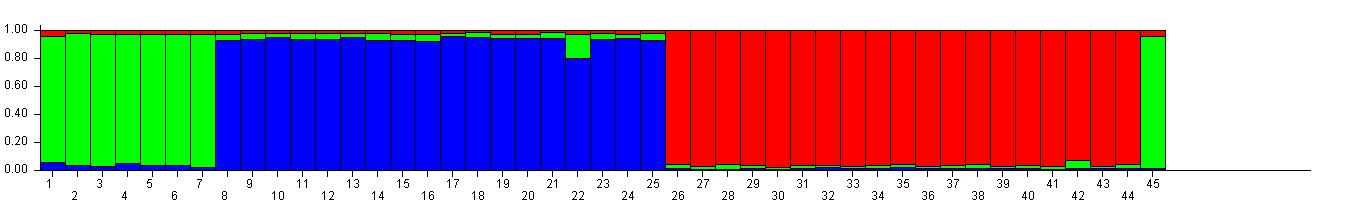
\includegraphics{/home/mrinalmanu/Desktop/pop_gen_hws/hw_2/panda_pops/k_3.jpg}
\caption{image}
\end{figure}

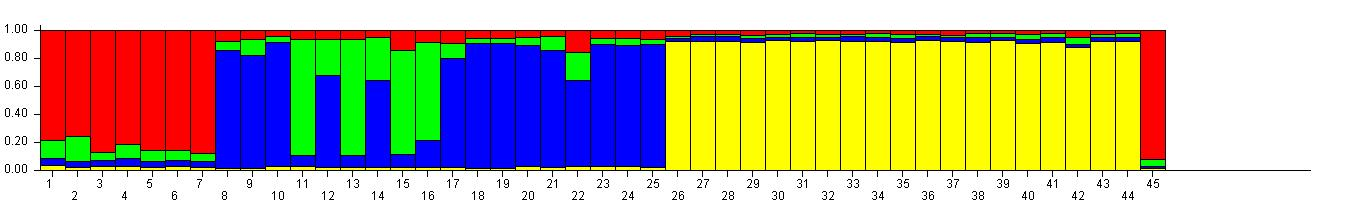
\includegraphics{//home/mrinalmanu/Desktop/pop_gen_hws/hw_2/panda_pops/k_4.jpg}
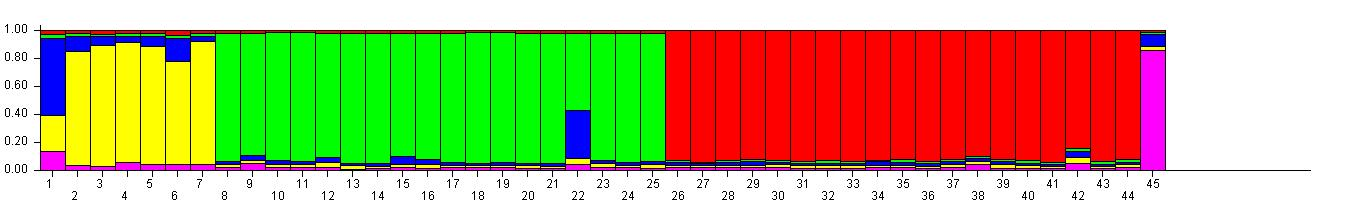
\includegraphics{/home/mrinalmanu/Desktop/pop_gen_hws/hw_2/panda_pops/k_5.jpg}

Clearly for 5 clusters we can see that one unique cluster pops out. Most
likely this is Giant Panda as mentioned in the oringal paper.

In all three images (k=3,4,and 5), the cluster for Polar bears remain
distinct. In other words the clustral membership in Polar bear cluster
remains exclusive. They are also homogenous in comparison, as suggested
by the findings in original paper.

\begin{figure}
\centering
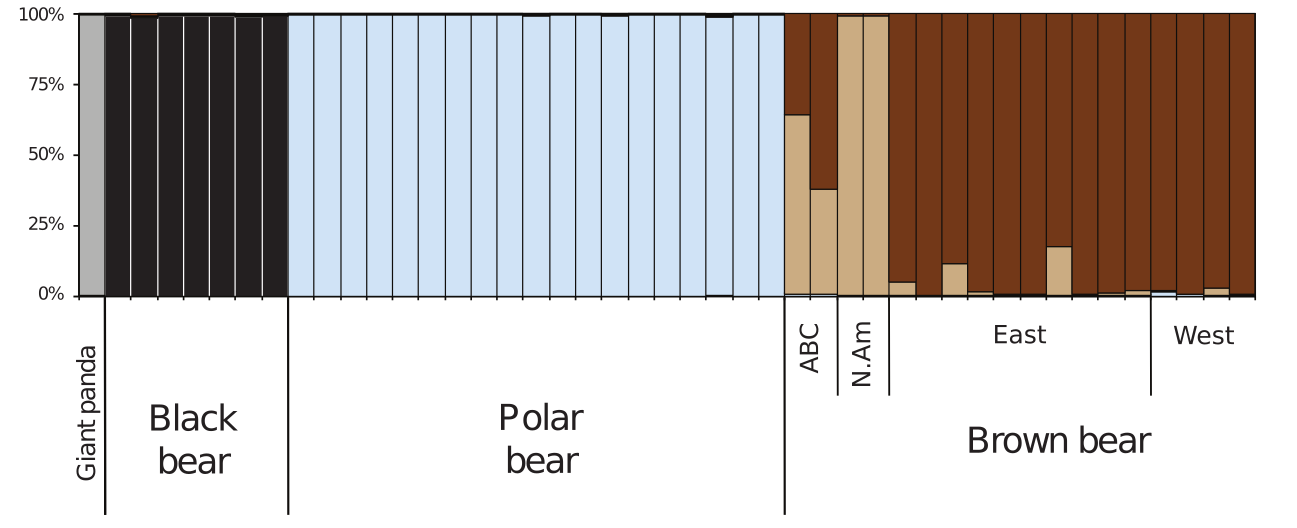
\includegraphics{/home/mrinalmanu/Desktop/pop_gen_hws/hw_2/main.png}
\caption{image}
\end{figure}

\hypertarget{soln-4}{%
\section{Soln 4}\label{soln-4}}

Lets draw the skyline plot for these parameters:

\begin{Shaded}
\begin{Highlighting}[]
\KeywordTok{library}\NormalTok{(ape)}
\end{Highlighting}
\end{Shaded}

\begin{verbatim}
## Warning: package 'ape' was built under R version 3.6.1
\end{verbatim}

\begin{Shaded}
\begin{Highlighting}[]
\KeywordTok{library}\NormalTok{(ggplot2)}
\end{Highlighting}
\end{Shaded}

\begin{verbatim}
## Warning: package 'ggplot2' was built under R version 3.6.1
\end{verbatim}

\begin{Shaded}
\begin{Highlighting}[]
\NormalTok{z <-}\StringTok{ }\KeywordTok{coalescent.intervals}\NormalTok{(}\KeywordTok{c}\NormalTok{(}\DecValTok{6000}\NormalTok{,}\DecValTok{2500}\NormalTok{,}\DecValTok{1000}\NormalTok{))}
\KeywordTok{skylineplot}\NormalTok{(z)}
\end{Highlighting}
\end{Shaded}

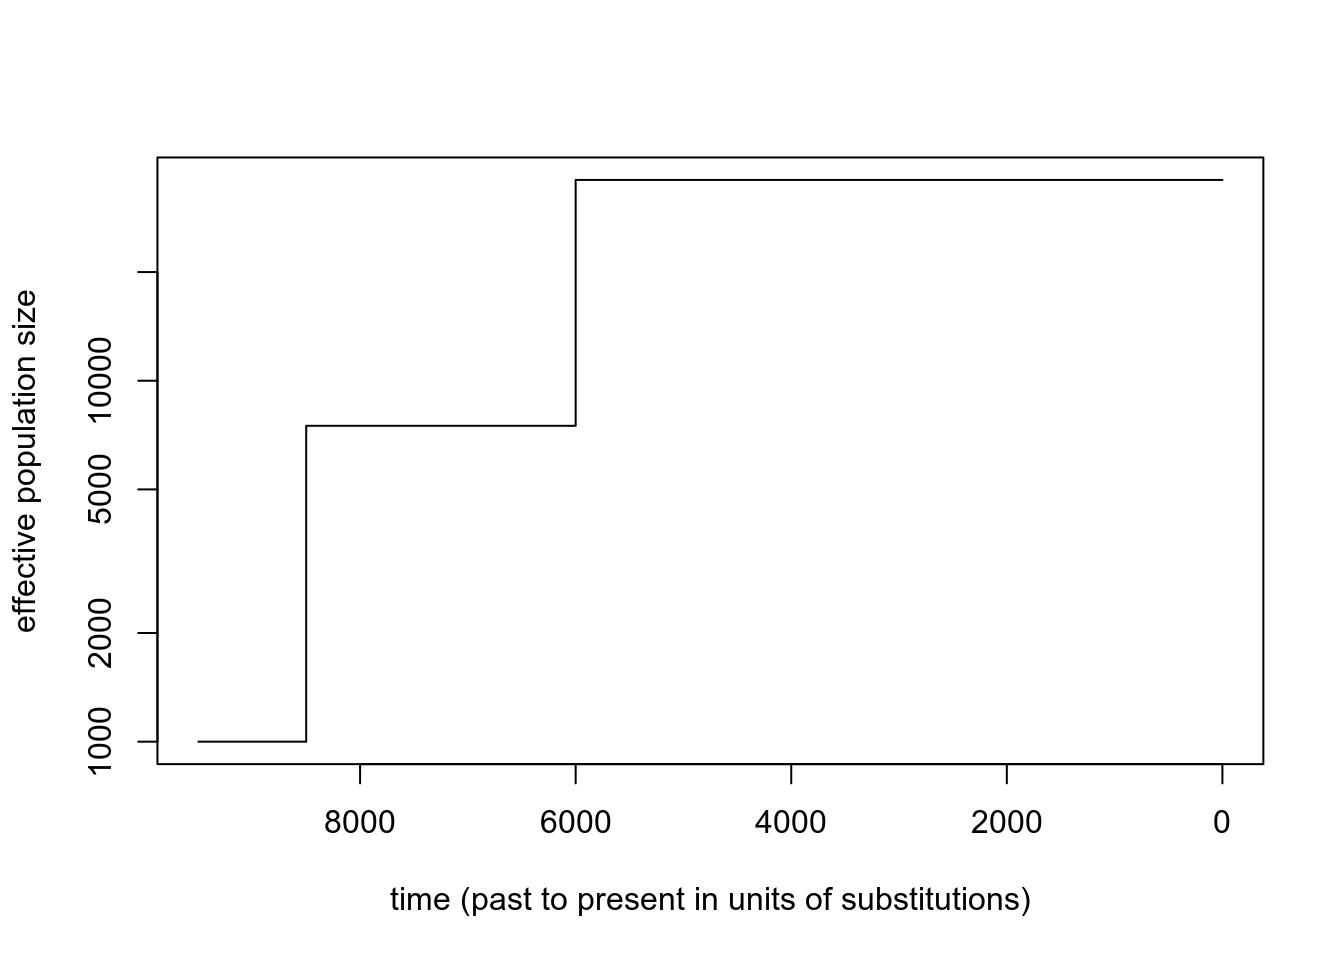
\includegraphics{hw_2_files/figure-latex/unnamed-chunk-1-1.pdf}

Here, the effective population size is increasing from past to present.
The population size has been increasing since last time 6000 years ago

\hypertarget{soln-4-1}{%
\section{Soln 4}\label{soln-4-1}}

Questions: 1) What is the (approximately) median log of posterior
probability as shown by Tracer? Please provide the plot of the
distribution.

around -27825, as written in the statistics column.

\begin{figure}
\centering
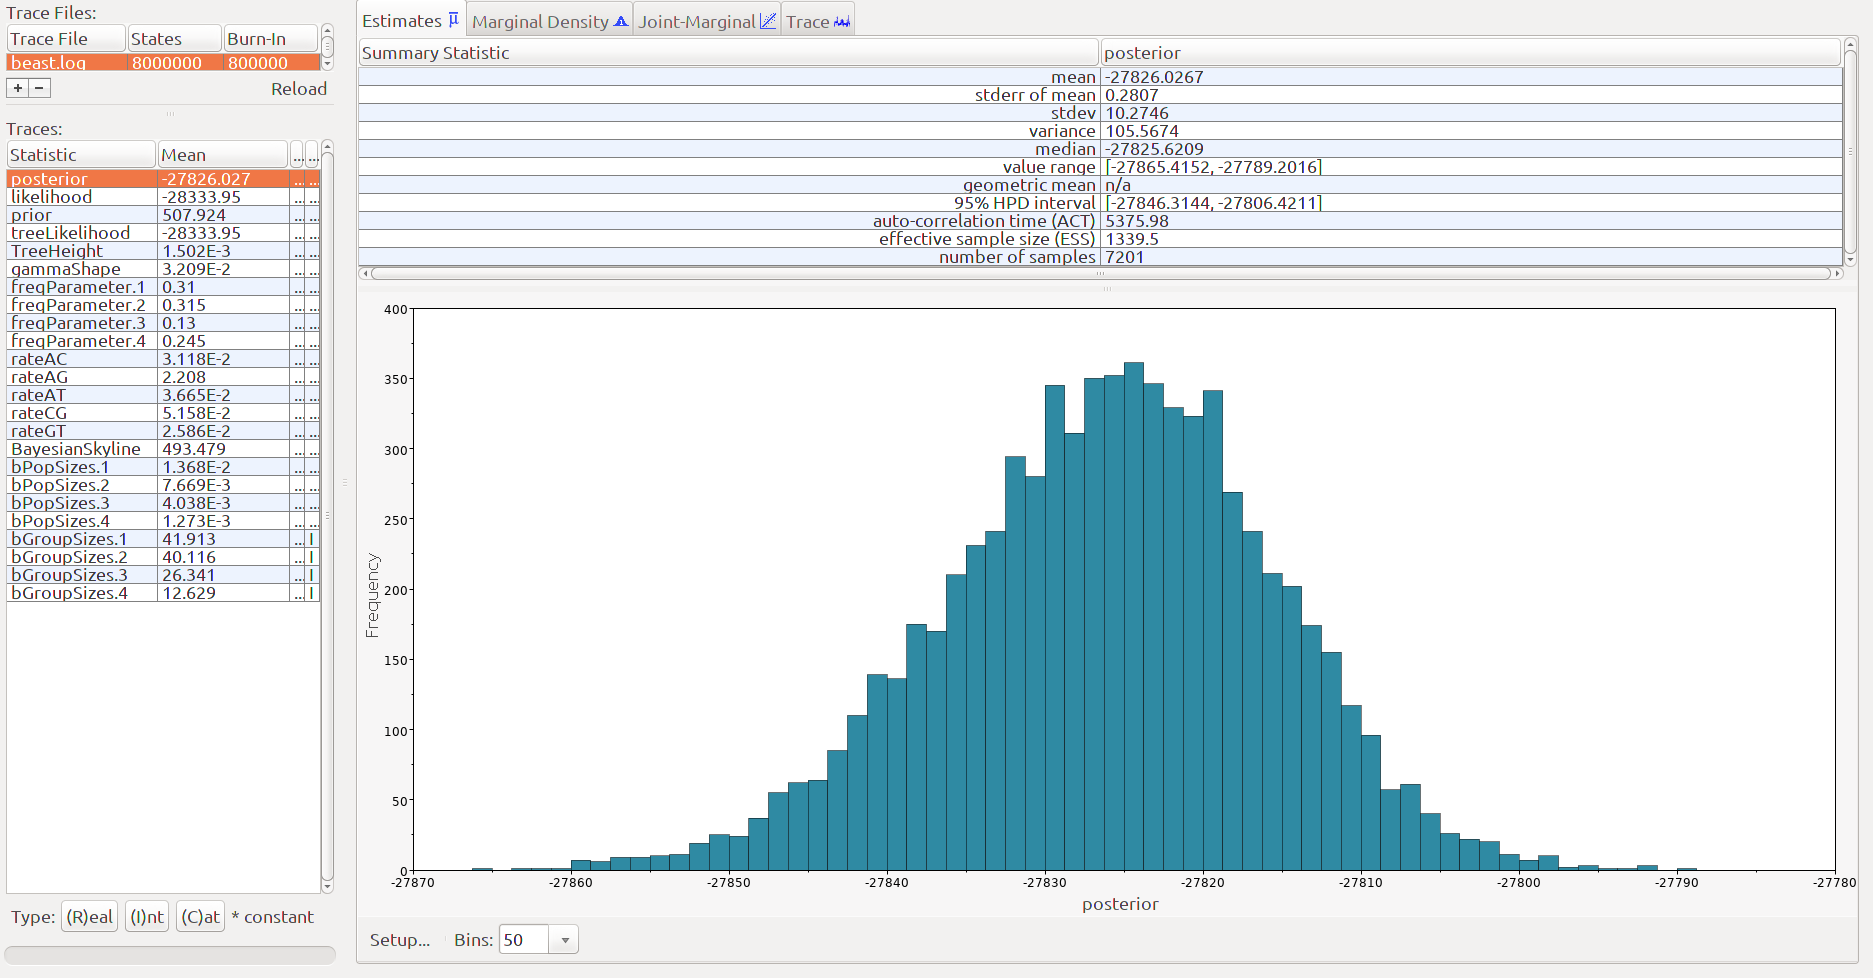
\includegraphics{/home/mrinalmanu/Desktop/pop_gen_hws/hw_2/vot.png}
\caption{image}
\end{figure}

\begin{enumerate}
\def\labelenumi{\arabic{enumi})}
\setcounter{enumi}{1}
\tightlist
\item
  How does the population size change over time? Were there any
  bottlenecks? Please provide the skyline plot.
\end{enumerate}

The population has a slow growth. At the end it seems like a bottleneck,
as can be seen in the skyline plot.

\begin{figure}
\centering
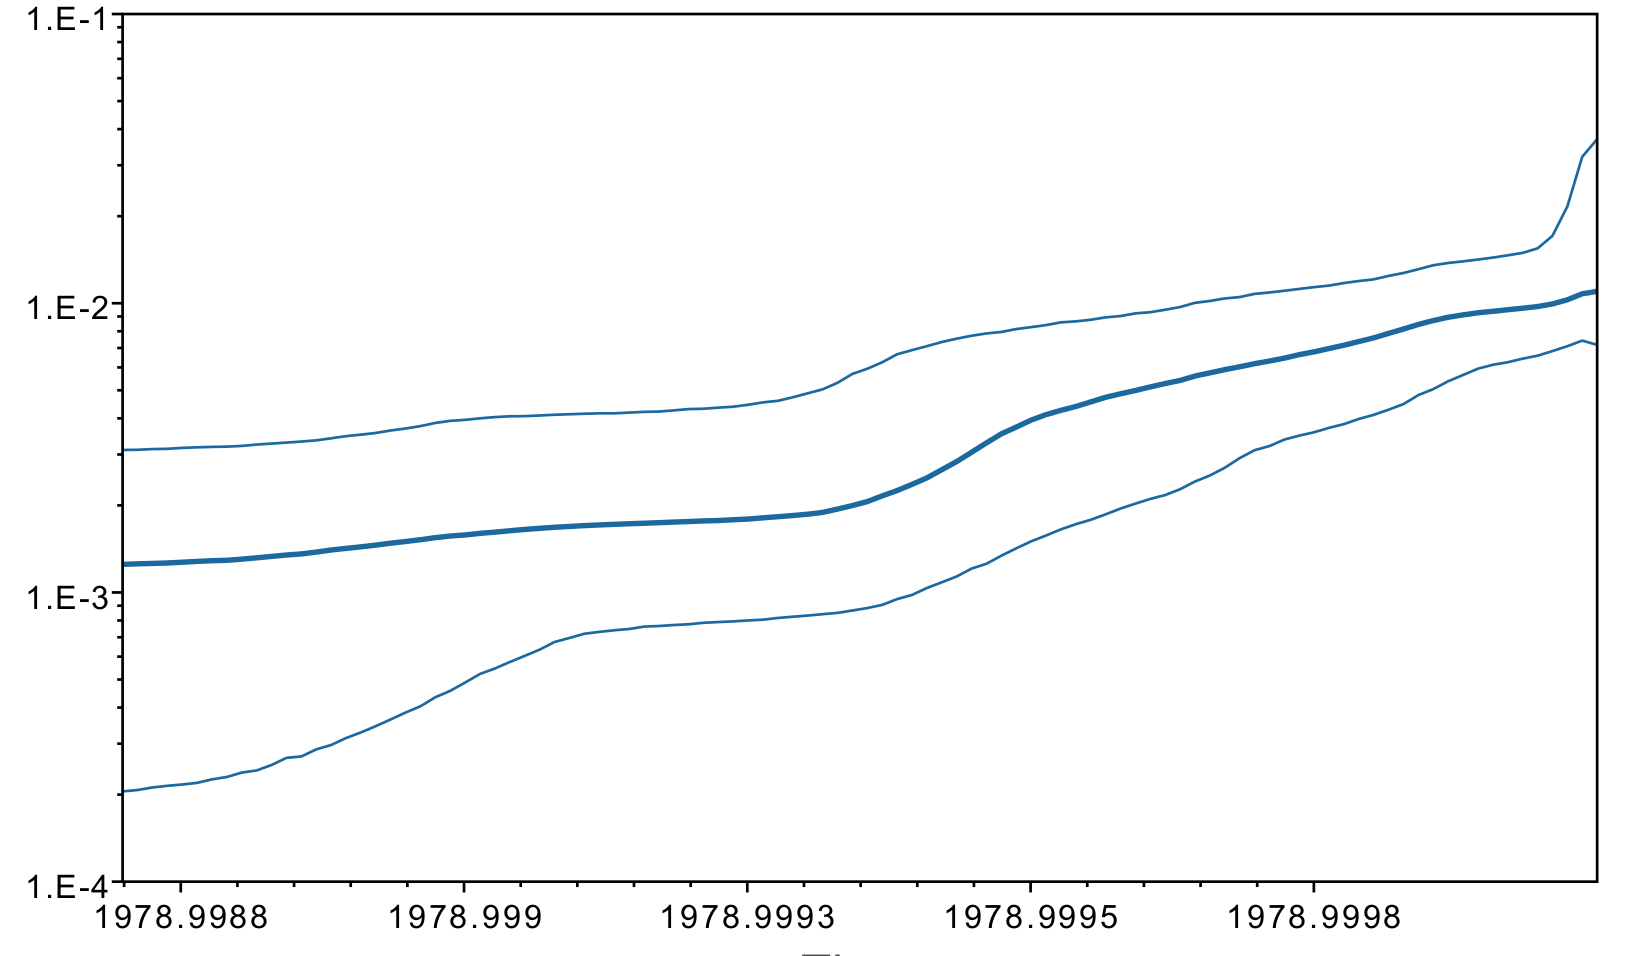
\includegraphics{/home/mrinalmanu/Desktop/pop_gen_hws/hw_2/skyline.png}
\caption{image}
\end{figure}

\begin{enumerate}
\def\labelenumi{\arabic{enumi})}
\setcounter{enumi}{2}
\tightlist
\item
  Compare your results with plots from the original paper. Which
  population was used in your analysis? Are there any differences in N e
  values?
\end{enumerate}

It seems like Sub-saharan population was used in our analysis.

Overall, N e values seem to be in the same magnitude.


\end{document}
